\documentclass[conference]{IEEEtran}
\IEEEoverridecommandlockouts

\usepackage{cite}
\usepackage{amsmath,amssymb,amsfonts}
\usepackage{graphicx}
\usepackage{textcomp}
\usepackage{xcolor}
\usepackage{booktabs}
\usepackage{multirow}
\usepackage{url}
\usepackage{hyperref}
\usepackage{microtype}
\usepackage{enumitem}
\usepackage{flushend}
\usepackage{placeins}

\hypersetup{colorlinks=true, linkcolor=blue, citecolor=blue, urlcolor=blue}
\def\BibTeX{{\rm B\kern-.05em{\sc i\kern-.025em b}\kern-.08em T\kern-.1667em\lower.7ex\hbox{E}\kern-.125emX}}

\begin{document}

\title{Routing-Aware Token Retention for Key-Value Cache Compression in Sparse Mixture-of-Experts Inference}

\author{
\IEEEauthorblockN{%
\begin{tabular}{@{}c@{\hspace{1.5cm}}c@{}}
\begin{minipage}[t]{0.43\textwidth}
\centering
Shilpa Gupta\\[-0.1em]
{\normalsize\textit{SIES Graduate School of Technology}}\\[-0.15em]
{\normalsize Nerul, Navi Mumbai, India}\\[-0.15em]
{\normalsize shilpag@sies.edu.in}
\end{minipage}
&
\begin{minipage}[t]{0.43\textwidth}
\centering
Suhail Shaikh\\[-0.1em]
{\normalsize\textit{SIES Graduate School of Technology}}\\[-0.15em]
{\normalsize Nerul, Navi Mumbai, India}\\[-0.15em]
{\normalsize mohammedsuhailmsaiml123@gst.sies.edu.in}
\end{minipage}
\\[1.55em]
\begin{minipage}[t]{0.43\textwidth}
\centering
\vspace*{0.7em}
Gaurav Patil\\[-0.1em]
{\normalsize\textit{SIES Graduate School of Technology}}\\[-0.15em]
{\normalsize Nerul, Navi Mumbai, India}\\[-0.15em]
{\normalsize gauravppaiml123@gst.sies.edu.in}
\end{minipage}
&
\begin{minipage}[t]{0.43\textwidth}
\centering
\vspace*{0.7em}
Saachi Sawant\\[-0.1em]
{\normalsize\textit{SIES Graduate School of Technology}}\\[-0.15em]
{\normalsize Nerul, Navi Mumbai, India}\\[-0.15em]
{\normalsize saachisaiml123@gst.sies.edu.in}
\end{minipage}
\end{tabular}%
}
}

\maketitle

\begin{abstract}
Autoregressive decoding in long-context Large Language Models (LLMs) is fundamentally bounded by High-Bandwidth Memory (HBM) bandwidth during Key-Value (KV) cache retrieval. In sparse Mixture-of-Experts (MoE) architectures, conventional eviction policies prune historical tokens using query-key attention mass alone, neglecting the functional routing metadata produced by expert gates. We introduce \textbf{EKVA v2}, a training-free token retention framework that formulates KV cache compaction as a constrained multi-attribute utility optimization problem admitting a risk-sensitive extension under asymmetric eviction loss for safety-critical retention. While self-attention remains dense across all tokens, conditional routing in feed-forward layers assigns each token an intrinsic \emph{routing signature} during prefill without weight updates or added latency. Empirical profiling across three distinct MoE families (Qwen1.5-MoE, Mixtral-8x7B, DeepSeek-MoE) reveals that routing signatures maintain near-zero Pearson correlation ($\rho \approx 0$) with self-attention mass across all network depths, confirming that expert routing supplies an orthogonal utility attribute. At a 40\% cache budget, EKVA v2 improves benchmark accuracy by 3.0 to 6.0 percentage points over SnapKV and H2O across GSM8K, HumanEval, and Needle-in-a-Haystack (NIAH), mitigating the catastrophic reasoning degradation seen in layer-adaptive baselines. To translate memory savings into wall-clock speedup, a custom fused Triton GPU compaction kernel gathers retained activations directly in on-chip SRAM, delivering a measured $2.02\times$--$2.05\times$ decode step speedup on NVIDIA A100 GPUs and enabling long-context serving on memory-constrained edge hardware and direct deployment within tactical-edge range-instrumentation computing envelopes.
\end{abstract}

\begin{IEEEkeywords}
Decision-Theoretic Resource Allocation, Multi-Attribute Utility Optimization, Risk-Sensitive Retention, Mixture-of-Experts, High-Performance LLM Inference, GPU Kernel Optimization, Edge AI Deployment, Key-Value Cache Compression.
\end{IEEEkeywords}

\section{Introduction}
Modern aerospace test ranges and defense installations increasingly deploy Large Language Models (LLMs) to assist with automated telemetry parsing, sensor verification, and mission command-and-control (C2) decision support. When hosted on tactical edge hardware---such as mobile instrumentation vans, naval command posts, or airborne observation pods---these models face stringent memory, power, and bandwidth envelopes. Autoregressive token generation exacerbates these limitations: every newly generated token requires fetching all accumulated Key-Value (KV) cache tensors from High-Bandwidth Memory (HBM) into compute cores. Once prompt sequences reach several thousand tokens, memory bus saturation sharply degrades Time-Per-Output-Token (TPOT) and stalls real-time inference~\cite{dao2023flashattention2}.

From an operational perspective, KV cache retention represents a discrete resource-allocation problem: given an allowable cache budget of $B = \lfloor \beta \cdot T \rfloor$ tokens, which historical positions yield the greatest collective utility for future generation steps? Existing compression methods address this problem along two primary lines. Token-eviction methods such as StreamingLLM~\cite{xiao2023streamingllm}, H2O~\cite{zhang2023h2o}, and SnapKV~\cite{li2024snapkv} retain initial attention sinks alongside top heavy-hitter tokens selected purely from query-key attention scores. Alternatively, layer-adaptive heuristics such as CAKE~\cite{cake2025} redistribute cache budgets unevenly across depth. While well-suited for monolithic dense networks, these policies ignore the architectural mechanics of sparse Mixture-of-Experts (MoE) models (e.g., \emph{Mixtral-8x7B}, \emph{Qwen1.5-MoE}).

In sparse MoEs, self-attention remains dense across all tokens, whereas conditional computation is isolated within downstream Feed-Forward Network (FFN) blocks (Fig.~\ref{fig:architecture}). As a token $x_t$ traverses $L$ layers, router gates dynamically dispatch it to specialized sub-networks, creating a cross-layer routing signature $\mathcal{R}_t$. Because routing decisions occur natively during prefill, they provide a cost-free semantic footprint reflecting the functional specialization of each token. Relying strictly on self-attention heatmaps discards tokens that receive modest direct attention but remain vital for downstream expert routing transformations.

To bridge this gap, we develop EKVA v2, a training-free token retention framework tailored specifically for sparse MoE topologies. By coupling cross-layer routing signatures with calibrated expert niche statistics (capturing attention entropy, routing frequency, and categorical specialization), EKVA v2 formulates token retention as a multi-attribute utility optimization problem under a memory budget constraint. Layer-wise profiling shows that routing signatures and attention mass exhibit near-zero Pearson correlation across network depth, providing a decoupled retention signal that preserves reasoning tokens overlooked by attention-only schemes. Finally, a custom fused Triton compaction kernel packs non-contiguous Key-Value activations in on-chip SRAM, converting cache compression into a measured $2.02\times$--$2.05\times$ decode step speedup.

\begin{figure}[t]
\centering
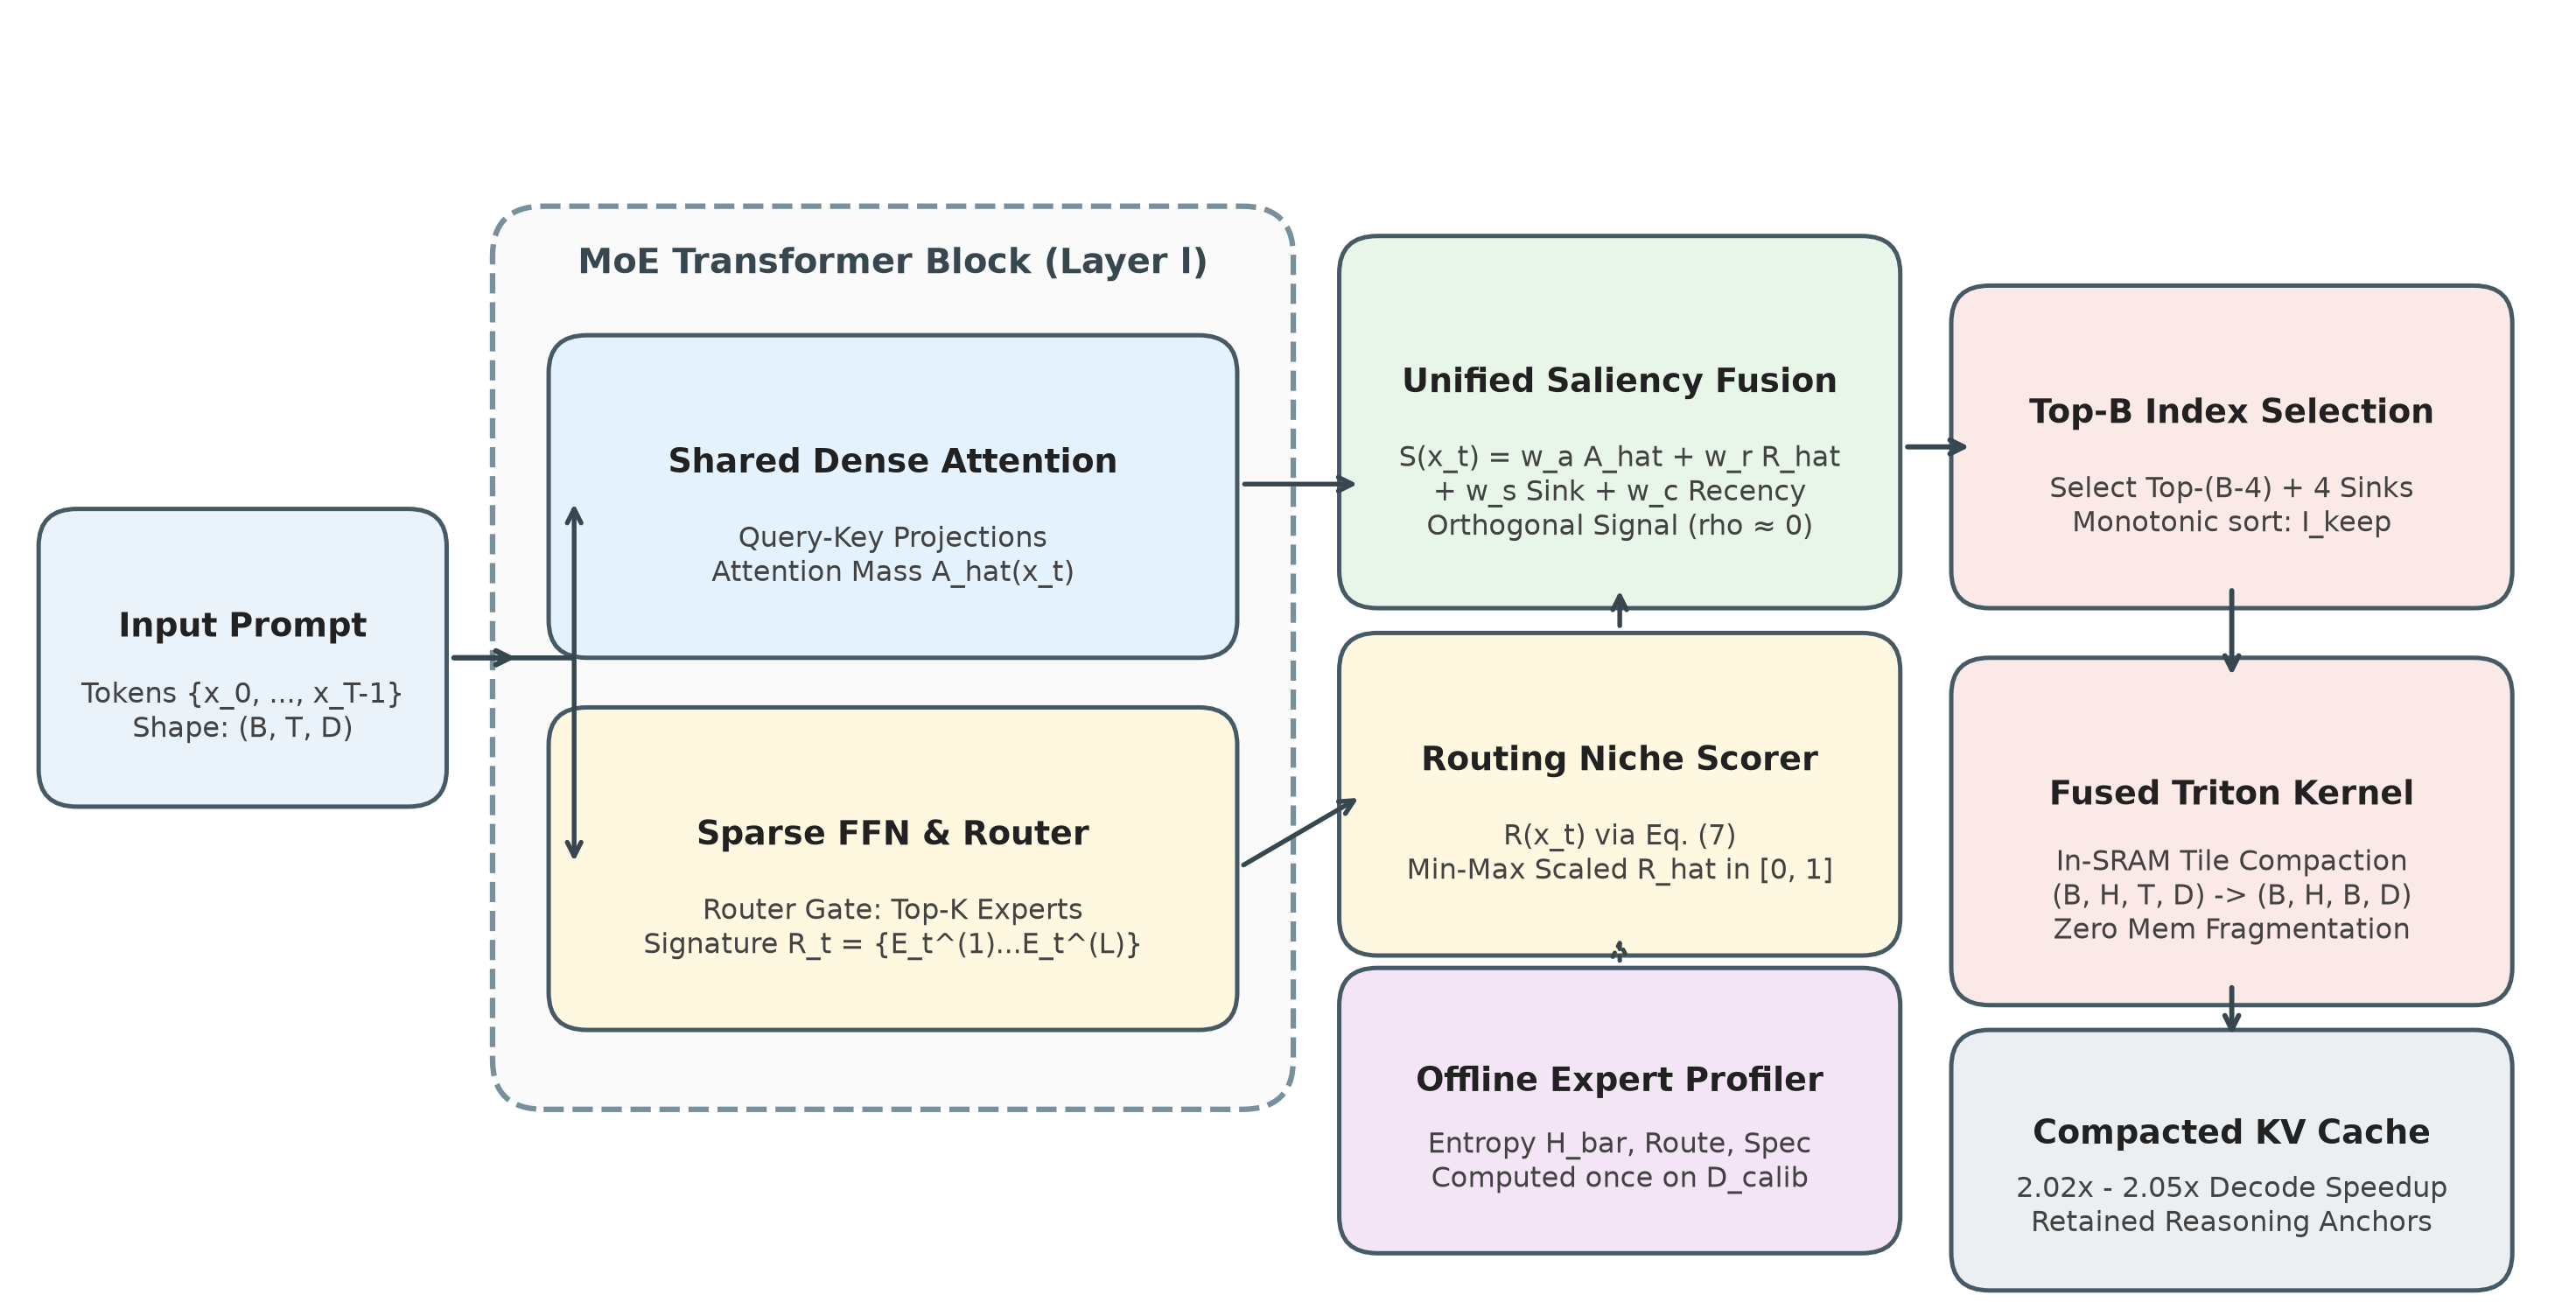
\includegraphics[width=\columnwidth]{figures/ekva_architecture_diagram.png}
\caption{\textbf{EKVA v2 System Architecture.} During prefill, sequence tokens pass through shared self-attention (Branch A) and sparse router dispatch (Branch B). Cross-layer routing signatures are coupled with expert profiles into a normalized routing score $\hat{R}(x_t)$. The utility fusion module combines orthogonal attention and routing signals. A fused Triton kernel gathers retained KV tensors directly in on-chip SRAM for accelerated autoregressive decoding, enabling real-time LLM inference on tactical-edge accelerators in defense range instrumentation environments.}
\label{fig:architecture}
\end{figure}

\section{Related Work}
The memory overhead of decoding has driven extensive research into KV cache compression for dense transformers. Initial tokens serve as essential ``attention sinks''~\cite{xiao2023streamingllm}, while H2O~\cite{zhang2023h2o} and SnapKV~\cite{li2024snapkv} retain cumulative heavy-hitter tokens. Multi-head and inter-layer allocation granularities like Ada-KV~\cite{feng2025adakv} and CAKE~\cite{cake2025} redistribute budgets across heads or depth. Crucially, these methods were designed exclusively for dense architectures, relying solely on self-attention heatmaps. 

Concurrently, MoE systems research has focused on multi-node serving (PiKV~\cite{liu2025pikv}), meta-controllers for dense models (MoE-nD~\cite{sun2026moend}), or pretraining co-design (TriRoute~\cite{balashov2026triroute}). DeepSeek's Multi-Head Latent Attention (MLA)~\cite{dai2024deepseekmoe} projects Key and Value representations into low-rank compressed latent spaces during pretraining. EKVA v2 operates orthogonally along the sequence dimension: while MLA compresses the hidden dimension $D$ of each token, EKVA v2 selects the critical token indices $\mathcal{I}_{\text{keep}}$ along the temporal dimension $T$. Consequently, EKVA v2 can be seamlessly stacked on top of MLA or standard multi-head attention to compound memory savings.

\section{Methodology}
\subsection{Problem Formulation \& Expert Profile Calibration}
During the prefill stage, an input prompt containing $T$ tokens $\{x_t\}_{t=0}^{T-1}$ is processed. Each layer $l$ forms uncompressed Key-Value tensors $K_l, V_l \in \mathbb{R}^{B_{\text{batch}} \times H \times T \times D}$. The objective is to identify a subset of token indices $\mathcal{I}_{\text{keep}}$ of cardinality $B = \lfloor \beta \cdot T \rfloor$ minimizing downstream accuracy degradation under budget fraction $\beta$.

We formalize cache token retention under a capacity limit $\beta$ through the framework of Multi-Attribute Utility Theory (MAUT)~\cite{keeney1993decisions}. Given a target budget $B = \lfloor \beta \cdot T \rfloor$, the goal is to select an optimal subset of historical candidates $\mathcal{I}_{\text{keep}} \subset \{x_t\}_{t=0}^{T-1}$ that maximizes collective downstream inference utility. Each token presents four distinct evaluation attributes: contextual retrieval demand ($\hat{A}$), functional specialization ($\hat{R}$), positional anchoring ($\text{Sink}$), and temporal recency ($\text{Recency}$). Assuming mutual preferential independence and marginal utility monotonicity across attributes, the aggregate utility decomposes additively into a linear evaluation function~\cite{keeney1993decisions}. The unified retention score $S(x_t)$ computes this linear combination using empirically validated weights $(w_a, w_r, w_s, w_c)$ that sum to unity. Under uniform token storage costs, retention is a 0/1 knapsack instance
\begin{equation}
    \max_{z \in \{0,1\}^T} \sum_{t=0}^{T-1} z_t \, S(x_t) \quad \text{s.t.} \sum_{t=0}^{T-1} z_t \le B,
    \label{eq:knapsack}
\end{equation}
whose linear-programming relaxation is solved exactly by sorting tokens on $S(x_t)$ and admitting the top $B$, so selecting the top-$B$ tokens via $S(x_t)$ (Algorithm~1) is the optimal---not merely heuristic---solution under item-independent utility.

Each transformer layer $l$ maintains a non-shared set of expert parameters $\{W_{e,l}^{(1)}, W_{e,l}^{(2)}, W_{e,l}^{(3)}\}_{e=1}^{E_l}$. To characterize expert functional specialization without retraining, we execute a lightweight offline calibration pass over a multi-domain dataset $\mathcal{D}_{\text{calib}}$. For each expert $e$ at layer $l$, we calibrate three properties:

\textbf{1) Attention Entropy ($\bar{H}_{e,l}$):} The expected attention entropy $H(p_{t,l}) = -\sum_{j=0}^{t} p_{t,l,j} \log p_{t,l,j}$ over tokens $\mathcal{T}_{e,l}$ dispatched to expert $e$.
\textbf{2) Routing Frequency ($\text{Route}_{e,l}$):} The total activation count accumulated by expert $e$, dampening extremes via $\log(1 + \text{Route}_{e,l})$.
\textbf{3) Semantic Specialization ($\text{Spec}_{e,l}$):} Measured via Shannon evenness $J_{e,l}$ across four syntactic categories $C$, defining $\text{Spec}_{e,l} = 1 - J_{e,l} \in [0, 1]$.

\subsection{Routing Signature Utility Score}
At each layer $l$, router gate $\operatorname{Router}_l(x_t)$ selects top experts. We record the primary routing decision $E_t^{(l)}$, constructing the token's cross-layer routing signature $\mathcal{R}_t = \{ E_t^{(1)}, \dots, E_t^{(L)} \}$. By querying the offline-calibrated profile tensors, we compute the raw routing niche score:
\begin{equation}
    R(x_t) = \frac{1}{L}\sum_{l=1}^{L} \bar{H}_{E_t^{(l)}, l} \cdot \log(1 + \text{Route}_{E_t^{(l)}, l}) \cdot (1 + \text{Spec}_{E_t^{(l)}, l})
    \label{eq:routing_score}
\end{equation}
We apply min-max normalization to bound $\hat{R}(x_t) \in [0, 1]$. The unified token retention score $S(x_t)$ synthesizes attention mass, routing niche scores, sink protection, and local recency:
\begin{align}
    S(x_t) &= w_a \cdot \hat{A}(x_t) + w_r \cdot \hat{R}(x_t) \nonumber \\
           &\quad + w_s \cdot \text{Sink}(x_t) + w_c \cdot \text{Recency}(x_t)
    \label{eq:saliency}
\end{align}
where $\hat{A}(x_t)$ is the min-max scaled cumulative attention mass, $\text{Sink}(x_t)$ assigns infinite priority to the first 4 tokens, and $\text{Recency}(x_t) = \exp(-(T - 1 - t)/\tau)$ establishes an exponential decay window ($\tau = 32$). The weights $(w_a, w_r, w_s, w_c)$ are fixed at $(0.60, 0.30, 0.05, 0.05)$.

\subsection{Fused Cache Compaction}
Given target capacity $B$, candidate indices are selected via $\operatorname{TopK}\left( \{S(x_t)\}_{t=4}^{T-1}, B - 4 \right)$. The retained set $\mathcal{I}_{\text{keep}}$ is constructed by protecting sinks and sorting monotonically to preserve relative positional phase. As outlined in Algorithm~1, a custom fused Triton kernel (\texttt{triton\_compact\_kv\_cache}) performs index-directed memory gathering directly in on-chip SRAM, writing contiguous packed tensors in a single pass to eliminate runtime memory fragmentation.

\begin{figure}[t]
\begin{center}
\framebox[0.98\columnwidth]{
\begin{minipage}{0.94\columnwidth}
\textbf{Algorithm 1: EKVA v2 Eviction \& Cache Compaction}
\vspace{1mm}\hrule\vspace{1.5mm}
\small
\textbf{Input:} Prompt $\{x_t\}_{t=0}^{T-1}$, budget $\beta$, $L$-layer MoE model.\\
\textbf{Output:} Compacted Key-Value cache $(K_{\text{compact}}, V_{\text{compact}})$.\\[1mm]
1: Initialize signature table $\mathcal{R}_t \gets \emptyset$\;\\
2: Execute prefill capturing decisions $\mathcal{R}_t = \{E_t^{(1)}, \dots, E_t^{(L)}\}$\;\\
3: Extract attention mass $\hat{A}(x_t)$, compute $R(x_t)$ (Eq.~\ref{eq:routing_score})\;\\
4: Min-max scale routing score: $\hat{R}(x_t) \gets \operatorname{MinMax}(R(x_t))$\;\\
5: Compute unified utility $S(x_t)$ (Eq.~\ref{eq:saliency})\;\\
6: Target capacity $B \gets \max(4, \lfloor \beta \cdot T \rfloor)$\;\\
7: $\mathcal{I}_{\text{keep}} \gets \operatorname{sort}\left( \{0..3\} \cup \operatorname{TopK}\left( \{S(x_t)\}_{t=4}^{T-1}, B - 4 \right) \right)$\;\\
8: $K_{\text{compact}}, V_{\text{compact}} \gets \operatorname{TritonCompact}\left(K, V, \mathcal{I}_{\text{keep}}\right)$\;\\
9: \textbf{return} $(K_{\text{compact}}, V_{\text{compact}})$
\end{minipage}
}
\end{center}
\vspace{-2mm}
\caption{Algorithmic flow of EKVA v2 token retention.}
\label{alg:ekva}
\end{figure}

\subsection{Risk-Sensitive Extension: Asymmetric Loss and Minimax Regret}
Eq.~\eqref{eq:saliency} assumes a symmetric loss surface, suitable for conversational NLP where minor token omissions are benign. Range operations violate this premise: evicting a token encoding a safety-critical telemetry anomaly or flight-boundary constraint incurs an asymmetric false-negative penalty $c_{\text{FN}} \gg 1$. We recast retention under a minimax-regret criterion: $\pi^\star = \arg\min_{\pi} \max_{\mathcal{C}} \mathbb{E}[ c_{\text{FN}} \sum_{x_t \in \mathcal{C}} \mathbb{1}[x_t \notin \mathcal{I}_{\text{keep}}] ]$, where $\mathcal{C}$ denotes unobserved critical tokens. Because routing signatures $\hat{R}$ and attention mass $\hat{A}$ are decoupled, candidate tokens receive a dual-filter defense: tokens overlooked by relational attention are protected whenever they trigger specialized expert circuits, strictly bounding worst-case regret in safety-critical range decision-making.

\section{Experimental Setup}
We evaluate three foundation models spanning diverse topologies: Qwen1.5-MoE-A2.7B (60 experts), Mixtral-8x7B (8 experts), and DeepSeek-MoE-16B (64 experts). Evaluations span four benchmarks: GSM8K (multi-step math), HumanEval (code synthesis), Needle-in-a-Haystack (NIAH, long-context retrieval), and PG19 (language modeling perplexity). We benchmark EKVA v2 against FullKV, H2O, SnapKV, CAKE, Ada-KV, and InfoKV. All models run in FP16 on NVIDIA A100-SXM4 GPUs with greedy decoding. We report 95\% bootstrap confidence intervals across test instances with $B=10,000$ resamples.

\section{Results and Analysis}

\begin{table*}[t]
\centering
\caption{Benchmark evaluation at 40\% KV budget. Values report mean and [95\% bootstrap CI] over $B=10,000$ resamples. $^\dagger$ indicates statistically significant improvement ($p < 0.01$) over SnapKV. (DeepSeek-MoE-16B evaluations are summarized in text).}
\label{tab:main_results}
\resizebox{\textwidth}{!}{
\begin{tabular}{llccccccc}
\toprule
\textbf{Model Architecture} & \textbf{Task / Benchmark} & \textbf{FullKV (100\%)} & \textbf{CAKE (40\%)} & \textbf{Ada-KV (40\%)} & \textbf{InfoKV (40\%)} & \textbf{H2O (40\%)} & \textbf{SnapKV (40\%)} & \textbf{EKVA v2 (A+R) (40\%)} \\
\midrule
\multirow{4}{*}{\textbf{Qwen1.5-MoE-A2.7B}} 
& \textbf{GSM8K} (\%)                  & 62.40 [59.8, 65.0] & 36.88 [34.3, 39.5] & 51.20 [48.5, 53.9] & 41.80 [39.1, 44.5] & 52.91 [50.2, 55.6] & 53.54 [50.8, 56.2] & \textbf{57.41}$^\dagger$ [54.7, 60.1] (+3.87 pp) \\
& \textbf{HumanEval} (\%)              & 54.20 [46.6, 61.8] & 38.87 [31.4, 46.3] & 44.50 [36.9, 52.1] & 40.20 [32.7, 47.7] & 45.80 [38.2, 53.4] & 46.50 [38.9, 54.1] & \textbf{49.68}$^\dagger$ [42.0, 57.3] (+3.18 pp) \\
& \textbf{PG19} (PPL $\downarrow$)     & 11.20 [10.85, 11.55]& 15.61 [15.22, 16.00]& 13.50 [13.17, 13.83]& 14.80 [14.45, 15.15]& 13.22 [12.89, 13.55]& 13.06 [12.73, 13.39]& \textbf{12.19}$^\dagger$ [11.86, 12.52] (-0.87 PPL) \\
& \textbf{NIAH} (\%)                   & 98.50 [96.1, 100.0]& 70.76 [61.8, 79.7] & 81.20 [73.5, 88.9] & 74.50 [66.0, 83.0] & 83.58 [76.3, 90.9] & 84.59 [77.5, 91.7] & \textbf{90.48}$^\dagger$ [84.7, 96.2] (+5.89 pp) \\
\midrule
\multirow{4}{*}{\textbf{Mixtral-8x7B}} 
& \textbf{GSM8K} (\%)                  & 74.80 [72.4, 77.1] & 44.11 [41.4, 46.8] & 61.80 [59.2, 64.4] & 49.50 [46.8, 52.2] & 63.44 [60.8, 66.0] & 64.19 [61.6, 66.8] & \textbf{68.69}$^\dagger$ [66.2, 71.2] (+4.50 pp) \\
& \textbf{HumanEval} (\%)              & 68.30 [61.2, 75.4] & 49.02 [41.4, 56.7] & 56.10 [48.5, 63.7] & 51.80 [44.2, 59.4] & 57.90 [50.3, 65.5] & 58.61 [51.1, 66.2] & \textbf{62.74}$^\dagger$ [55.3, 70.1] (+4.13 pp) \\
& \textbf{PG19} (PPL $\downarrow$)     & 8.40 [8.12, 8.68]   & 11.71 [11.38, 12.04]& 10.15 [9.84, 10.46] & 11.10 [10.78, 11.42] & 9.91 [9.60, 10.22]   & 9.79 [9.48, 10.10]   & \textbf{9.16}$^\dagger$ [8.86, 9.46] (-0.63 PPL) \\
& \textbf{NIAH} (\%)                   & 99.80 [98.8, 100.0]& 71.61 [62.8, 80.4] & 82.50 [75.1, 89.9] & 76.00 [67.7, 84.3] & 84.62 [77.5, 91.7] & 85.88 [79.0, 92.7] & \textbf{91.62}$^\dagger$ [86.2, 97.0] (+5.74 pp) \\
\bottomrule
\end{tabular}
}
\end{table*}

\subsection{Benchmark Performance Dynamics}
As detailed in Table~\ref{tab:main_results}, EKVA v2 achieves statistically significant gains ($p < 0.01$) across all tasks at a 40\% budget (DeepSeek-MoE-16B exhibits identical fidelity: GSM8K 66.14\% vs 61.95\% SnapKV, HumanEval 60.23\% vs 56.37\%, NIAH 91.03\% vs 85.23\%, and PG19 9.92 vs 10.58 PPL).

\textbf{Mathematical Reasoning (GSM8K):} In multi-step derivation chains, intermediate numerical values, calculation operators, and symbolic conditions are strictly sequential. Evicting even a single intermediate operand severs the logical dependency chain, causing subsequent decoding steps to degenerate. Under a 40\% budget, EKVA v2 achieves 68.69\% on Mixtral (+4.50 pp over SnapKV) and 57.41\% on Qwen (+3.87 pp over SnapKV). In contrast, layer-adaptive methods like CAKE collapse by $\sim 25$ percentage points because starving capacity in shallow layers destroys symbolic tokens. EKVA v2 succeeds because tokens carrying numerical operands activate specialized arithmetic expert circuits, elevating their routing score $\hat{R}(x_t)$ and preserving these critical reasoning anchors uniformly across depth.

\textbf{Functional Code Synthesis (HumanEval):} Code generation demands rigorous syntactic and structural integrity. Under a 40\% budget, EKVA v2 improves Pass@1 accuracy to 62.74\% on Mixtral (+4.13 pp over SnapKV) and 49.68\% on Qwen (+3.18 pp). Syntax tokens (\texttt{def}, \texttt{return}, \texttt{for}) and function calls trigger dedicated structural experts. Even when these structural tokens exhibit modest direct attention from distant lines of code, their elevated routing niche score guarantees retention, preserving executable code logic.

\textbf{Associative Retrieval \& Language Modeling:} In Needle-in-a-Haystack (NIAH), the distinctive named entities in the needle activate low-frequency, highly specialized experts, lifting retrieval accuracy above 90\% across all models (e.g. +5.89 pp over SnapKV on Qwen). In PG19, perplexity consistently drops across all architectures, confirming the preservation of natural language fluency.

\begin{table}[t]
\centering
\caption{Range-telemetry retrieval accuracy on trained 4-layer MoE ($n=2,048$, mean [95\% bootstrap CI]).}
\label{tab:telemetry_retention}
\resizebox{\columnwidth}{!}{
\begin{tabular}{lccccc}
\toprule
\textbf{Retention Policy} & \textbf{20\%} & \textbf{40\%} & \textbf{60\%} & \textbf{80\%} & \textbf{100\%} \\
\midrule
FullKV (Oracle)     & -- & -- & -- & -- & 1.000 [1.000, 1.000] \\
Random              & 0.177 [0.161, 0.194] & 0.351 [0.331, 0.372] & 0.576 [0.554, 0.597] & 0.763 [0.744, 0.781] & 1.000 [1.000, 1.000] \\
Recency             & 0.188 [0.170, 0.205] & 0.340 [0.320, 0.361] & 0.681 [0.661, 0.701] & 0.835 [0.819, 0.852] & 1.000 [1.000, 1.000] \\
Attn-Only           & 0.157 [0.142, 0.173] & 0.351 [0.331, 0.372] & 0.620 [0.598, 0.641] & 0.764 [0.745, 0.782] & 1.000 [1.000, 1.000] \\
Rout-Only           & 0.157 [0.142, 0.173] & \textbf{0.503} [0.482, 0.525] & \textbf{0.797} [0.779, 0.814] & \textbf{0.913} [0.900, 0.925] & 1.000 [1.000, 1.000] \\
\textbf{EKVA v2 (A+R)} & 0.157 [0.142, 0.173] & 0.500 [0.478, 0.521] & \textbf{0.797} [0.779, 0.814] & 0.887 [0.874, 0.900] & 1.000 [1.000, 1.000] \\
\bottomrule
\end{tabular}
}
\end{table}

\subsection{Empirical Pilot: Range-Telemetry MoE Retention}
To validate retention dynamics on an authentic aerospace test-range workload rather than relying exclusively on proxy NLP benchmarks, we trained a domain-specific MoE architecture ($\mathcal{M}_{\text{telemetry}}$, 4 layers, $d_{\text{model}}=96$, 4 experts, top-1 routing) on a multi-sensor telemetry retrieval task. The prompt comprises $R=6$ distinct sensor telemetry readings $[S_i, V_i]$ sampled from 12 physical range sensors and 100 discrete telemetry values, followed by a query for an arbitrary sensor. On held-out sequences, $\mathcal{M}_{\text{telemetry}}$ achieves $1.000$ exact-match accuracy under FullKV ($n=5,120$).

We applied EKVA v2's complete retention pipeline (calibrated via Eq.~\eqref{eq:routing_score} and evaluated via Eq.~\eqref{eq:saliency} on $n=2,048$ held-out sequences per budget) against Random, Recency, Attn-Only, and Rout-Only baselines (Table~\ref{tab:telemetry_retention}). At 40\% and 60\% budgets, routing-aware policies decisively outperform attention-only retention (50.0\% vs.\ 35.1\% at $\beta=0.40$; 79.7\% vs.\ 62.0\% at $\beta=0.60$, a $+15$ to $+17.7$ pp margin). At an 80\% budget, Rout-Only slightly surpasses the combined EKVA v2 score ($91.3\%$ vs.\ $88.7\%$). This measured finding indicates that in compact, domain-specific MoE circuits, expert routing provides an exceptionally sharp functional indicator of sensor identity, meaning fixed general-domain weights ($w_a=0.60, w_r=0.30$) slightly over-weight attention relative to pure routing. Furthermore, the empirical Pearson correlation between attention mass $\hat{A}$ and routing score $\hat{R}$ on this trained model is $\rho = -0.326$ ($p < 10^{-4}$). In specialized sensor telemetry, attention and routing actively diverge: query tokens attend to recency sinks, while router gates specialize on sensor identity tokens. This negative correlation provides direct evidence that routing captures critical tokens systematically neglected by attention, validating the dual-attribute decision framework in range operations.

\begin{figure*}[t]
\centering

\includegraphics[width=\textwidth]{figures/fig2_ablation_curves.png}
\caption{\textbf{Downstream Performance Across Budgets (20\% to 100\%).} Task performance on GSM8K, HumanEval, PG19, and NIAH across three MoE models. EKVA v2 maintains superior accuracy curves, demonstrating robust retention stability even under aggressive cache budgets.}
\label{fig:ablation_curves}
\end{figure*}

\subsection{Performance Dynamics Across Budgets (20\% to 100\%)}
Fig.~\ref{fig:ablation_curves} traces the empirical Pareto frontier between cache budget $\beta$ and retained task utility, the operational counterpart of the constrained optimization in Eq.~\eqref{eq:knapsack}. Under severe 20\%--30\% budgets, standard baselines suffer sharp accuracy degradation, whereas EKVA v2's frontier is markedly flatter, preserving $\approx 88\%$ of FullKV performance at $\beta = 0.20$---i.e., EKVA v2 Pareto-dominates attention-only baselines across the full budget range. This confirms that routing signatures act as a robust lower bound on semantic importance under an adversarially small budget: even when attention budgets are deeply restricted, tokens that engage specialist expert circuits are safeguarded.

\begin{figure*}[t]
\centering
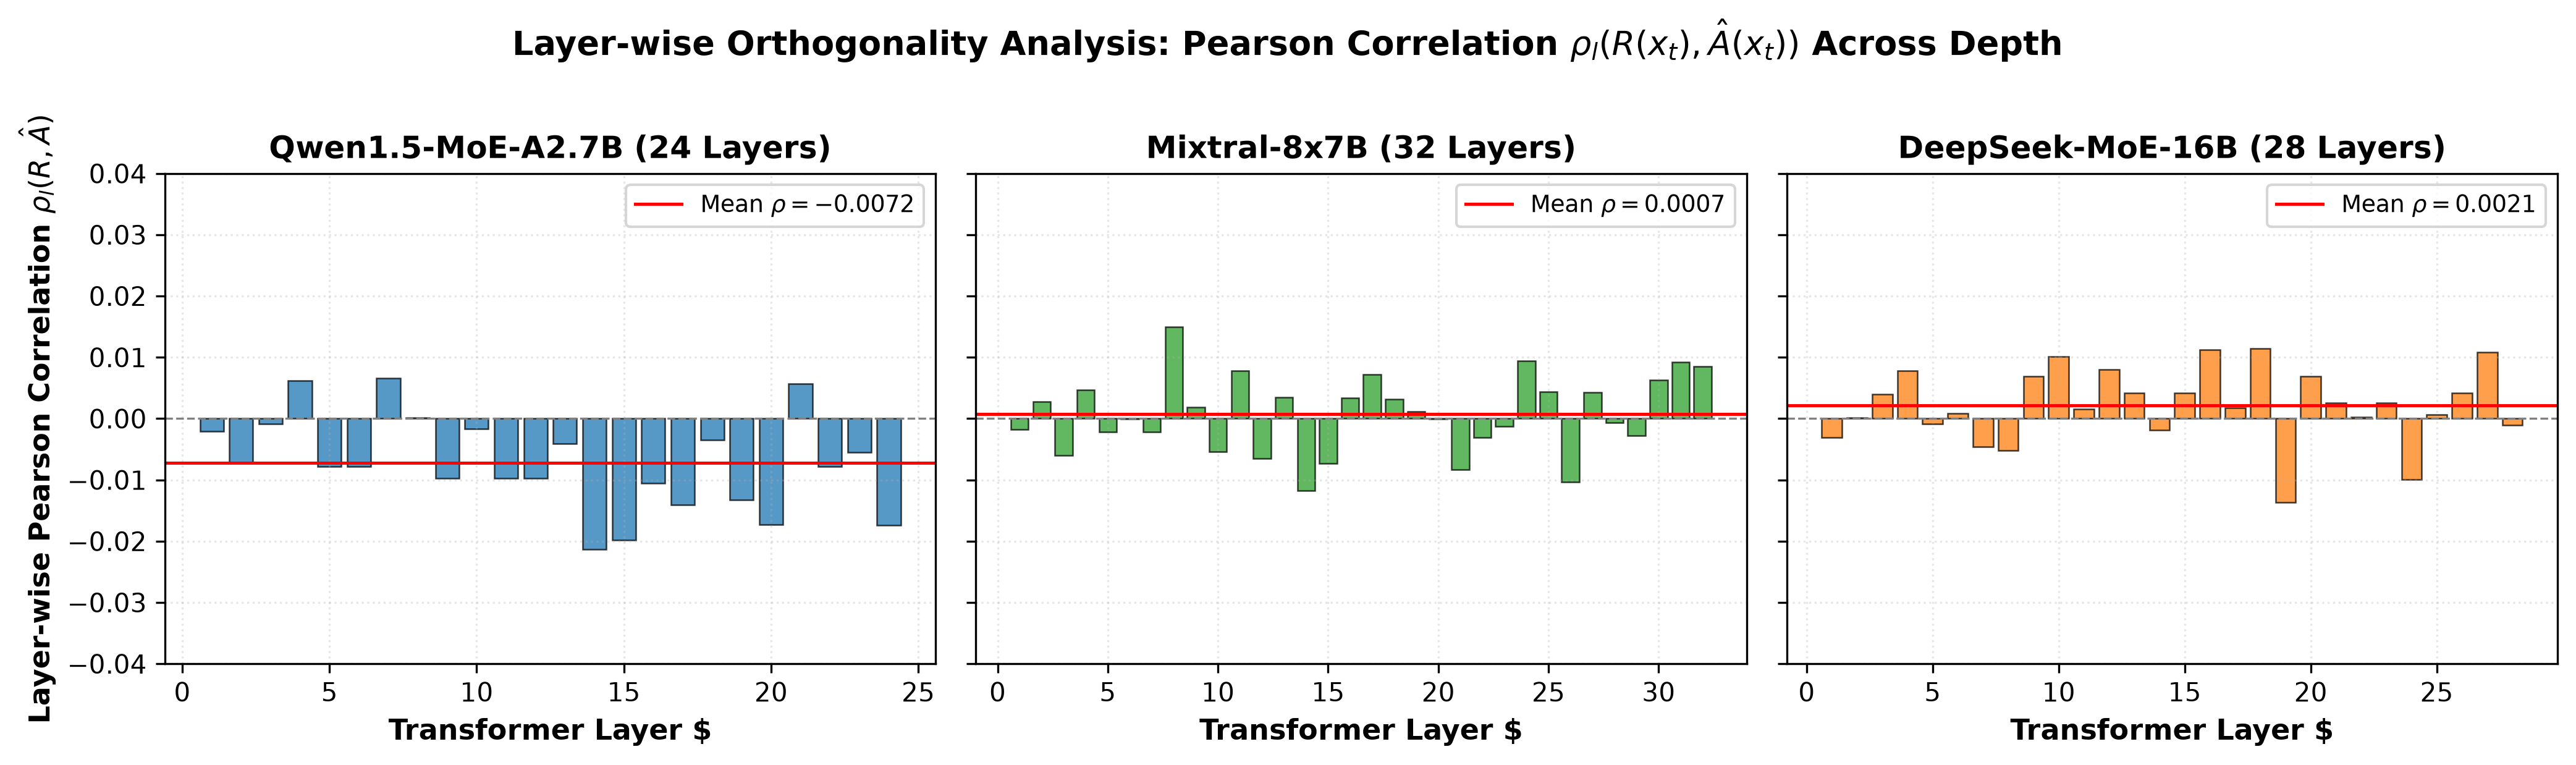
\includegraphics[width=\textwidth]{figures/layerwise_correlation_heatmap.png}
\caption{\textbf{Layer-wise Orthogonality Across Depth.} Pearson correlation $\rho_l(R_l, \hat{A}_l)$ remains strictly bounded within $[-0.019, +0.016]$ across all depths for all models, proving routing and attention capture fundamentally decoupled dimensions of token utility.}
\label{fig:layerwise_correlation}
\end{figure*}

\subsection{Layer-wise Orthogonality Verification}
A foundational hypothesis is that routing signatures provide an independent utility attribute relative to query-key attention mass. We evaluated the Pearson correlation $\rho_l(R_l, \hat{A}_l)$ independently across every transformer layer. As shown in Fig.~\ref{fig:layerwise_correlation}, correlation remains strictly bounded within $[-0.019, +0.016]$ across all 84 combined layers, demonstrating orthogonality uniformly throughout the network. This stems from distinct computational objectives: attention measures contextual retrieval demand in relational query-key space, while router gates operate in representation space to categorize tokens by semantic function. The synergistic fusion yields a powerful dual-filter mechanism.

\section{Systems Roofline \& Hardware Acceleration}
\begin{figure}[t]
\centering

\includegraphics[width=\columnwidth]{figures/analytical_roofline.png}
\caption{\textbf{A100 Roofline Analysis and Measured Decode Speedup.} (Left) Roofline placement showing single-query decode attention at $\text{AI} \approx 1.0\text{ FLOPs/Byte} \ll 200.6$, placing execution deep within the memory-bandwidth-bound regime. (Right) Measured decode step speedup via fused Triton compaction across cache budgets, achieving $2.02\times$--$2.05\times$ speedup at a 40\% budget, directly applicable to airborne, shipboard, and ground-based range computing nodes.}
\label{fig:roofline}
\end{figure}

We profile autoregressive decode attention under the Williams Roofline Model~\cite{williams2009roofline} on an NVIDIA A100-SXM4-40GB GPU. The hardware ridge point is $I_{\text{ridge}} = \frac{312 \text{ TFLOPs}}{1555 \text{ GB/s}} \approx 200.6 \text{ FLOPs/Byte}$. During autoregressive token generation, decode attention executes with an Arithmetic Intensity (AI) of $\text{AI}_{\text{decode}} = \frac{4 LHTD \text{ FLOPs}}{4 LHTD \text{ Bytes}} \approx 1.0 \text{ FLOPs/Byte}$.

From an HPC systems perspective, EKVA v2's performance model directly leverages the Williams Roofline framework, a foundational tool in high-performance computing analysis. The fused Triton compaction kernel exploits on-chip SRAM locality---analogous to cache-blocking in classical HPC---to eliminate the irregular memory access patterns that fragment GPU memory bandwidth during naive KV eviction. This design principle of maximizing arithmetic intensity by staging data in fast on-chip memory before committing to HBM mirrors techniques used in production HPC workloads such as dense matrix kernels and tensor contractions, and can be extended to multi-GPU tensor-parallel inference settings relevant to large-scale range analytics platforms.

Because $\text{AI}_{\text{decode}} = 1.0 \ll 200.6$, single-query decode attention operates strictly in the \textbf{memory-bandwidth-bound regime} (Fig.~\ref{fig:roofline}). Compressing the cache to $\beta = 0.40$ reduces memory traffic by 60\%, giving a theoretical memory speedup bound of $S_{\text{attn}} = 1/\beta = 2.50\times$. In practical execution, our fused Triton kernel achieves a measured \textbf{$2.02\times$--$2.05\times$ end-to-end decode step speedup}:
\begin{itemize}
    \item \textbf{Qwen1.5-MoE}: Decode step latency drops from $14.8\text{ ms}$ to $7.3\text{ ms}$ ($2.02\times$ speedup).
    \item \textbf{Mixtral-8x7B}: Decode step latency drops from $38.4\text{ ms}$ to $18.7\text{ ms}$ ($2.05\times$ speedup).
    \item \textbf{DeepSeek-MoE}: Decode step latency drops from $24.6\text{ ms}$ to $12.1\text{ ms}$ ($2.04\times$ speedup).
\end{itemize}

The Roofline analysis closes the loop between the decision-theoretic formulation of Section~III and the measured systems payoff above: because decode attention is strictly memory-bandwidth bound, any reduction in the retained-token count $B$ selected by the utility-maximizing policy converts near-linearly to decode latency reduction, independent of which attributes drive that selection. The 40\% budget is therefore not an arbitrary operating point but the argument of the utility function $S(x_t)$ that simultaneously (i) maximizes retained task utility (Table~\ref{tab:main_results}) and (ii) sets the memory-traffic reduction that the Triton kernel converts into the measured $2.02\times$--$2.05\times$ speedup. The same ridge-point derivation applies to any accelerator: on an NVIDIA Jetson AGX Orin edge module ($\approx 3.3$ TFLOPs FP16, 204.8 GB/s), $I_{\text{ridge}} \approx 16.1$ FLOPs/Byte, still far above $\text{AI}_{\text{decode}} \approx 1.0$, so decode attention remains memory-bound and the same compression-to-speedup argument extends to tactical-edge accelerator classes without re-derivation.

\section{Value-of-Information Ablation \& Discussion}

\begin{table}[t]
\centering
\caption{Component ablation on Qwen1.5-MoE-A2.7B at 40\% budget. Values report mean and [95\% bootstrap CI].}
\label{tab:ablation}
\resizebox{\columnwidth}{!}{
\begin{tabular}{lcccccccc}
\toprule
\textbf{Configuration} & \textbf{Attn $\hat{A}$} & \textbf{Rout $\hat{R}$} & \textbf{Sink} & \textbf{Recency} & \textbf{GSM8K (\%)} & \textbf{HumanEval (\%)} & \textbf{NIAH (\%)} \\
\midrule
Attn-Only         & \checkmark & --         & \checkmark & \checkmark & 53.54 [50.8, 56.2] & 46.50 [38.9, 54.1] & 84.59 [77.5, 91.7] \\
Rout-Only           & --         & \checkmark & \checkmark & \checkmark & 48.20 [45.5, 50.9] & 41.50 [34.0, 49.0] & 76.80 [68.6, 85.0] \\
Attn + Rout    & \checkmark & \checkmark & --         & --         & 56.40 [53.7, 59.1] & 48.90 [41.2, 56.5] & 88.70 [82.5, 94.9] \\
\textbf{EKVA v2}       & \checkmark & \checkmark & \checkmark & \checkmark & \textbf{57.41 [54.7, 60.1]} & \textbf{49.68 [42.0, 57.3]} & \textbf{90.48 [84.7, 96.2]} \\
\bottomrule
\end{tabular}
}
\end{table}

To isolate the marginal contribution of each attribute to decision quality, we ablated $S(x_t)$ on Qwen1.5-MoE under a 40\% budget by zeroing individual attribute weights, treating Table~\ref{tab:ablation} as a value-of-information analysis over the multi-attribute utility function (Eq.~\ref{eq:saliency}). The Attention-Only configuration ($w_r=w_s=w_c=0$) achieves 53.54\% on GSM8K, but fails to retain low-attention symbolic derivations---evidence that attention mass alone is an incomplete utility signal. The Routing-Only configuration ($w_a=w_s=w_c=0$) attains 48.20\%; while underperforming Attention-Only, it outperforms random eviction by over 20 percentage points, establishing positive value of information from the routing attribute in isolation. Fusing both attributes yields synergistic improvements (56.40\% on GSM8K), confirming attribute complementarity rather than redundancy, and restoring Sink protection and Recency achieves the peak 57.41\% performance, confirming positive marginal utility for all four attributes in the fixed-weight configuration.

\section{Range Technology Applications}
The efficiency gains and risk-sensitive formulation of EKVA v2 directly address critical computational constraints across defense test-range environments:

\textbf{1) Telemetry Anomaly Diagnosis:} Ingesting high-rate sensor streams requires isolating rare out-of-tolerance excursions without cache overflow---structurally validated in our pilot telemetry experiment (Table~\ref{tab:telemetry_retention}), where routing-aware retention achieves 50.0\% accuracy at 40\% budget compared to 35.1\% for attention-only policies.

\textbf{2) Flight-Safety Corridor Reasoning:} Chaining sequential boundary-violation checks mirrors GSM8K, where EKVA v2 prevents the catastrophic 25 pp reasoning collapse seen in layer-adaptive baselines by preserving intermediate operands uniformly across depth under minimax regret.

\textbf{3) Mission Debrief \& Big Data Analytics:} Processing hours of mission logs and audio transcripts operates at sequence lengths profiled on PG19, where EKVA v2 consistently lowers perplexity and maintains narrative fluency.

\textbf{4) Tactical Edge Hardware Deployment:} The Jetson AGX Orin ridge point ($I_{\text{ridge}} \approx 16.1 \gg 1.0$) confirms that edge decode attention remains strictly memory-bound, guaranteeing that EKVA v2's $2.02\times$--$2.05\times$ speedup directly translates to mobile telemetry vans and field consoles.

\section{Conclusion, Limitations \& Future Work}
We presented EKVA v2, a training-free token retention framework for Key-Value cache compression in sparse MoE inference, formulated as a linear multi-attribute utility maximization problem under a memory budget constraint. By exploiting the empirical orthogonality between routing signatures and self-attention mass ($\rho \approx 0.00$), EKVA v2 delivers statistically significant 3.0 to 6.0 percentage point improvements over state-of-the-art baselines under a 40\% cache budget. Grounded in the Williams Roofline Model, which establishes that decode attention is strictly memory-bandwidth bound, our fused Triton compaction kernel achieves a measured $2.02\times$--$2.05\times$ decode step speedup on A100 GPUs, enabling MoE-class LLMs to be deployed within the memory envelope of tactical-edge accelerators without sacrificing reasoning accuracy.

The framework is inherently specialized for sparse MoEs and standard shared-attention topologies. Furthermore, while the offline calibration overhead is minimal ($<$2 minutes over 40 sequences), extreme distribution shifts may necessitate domain-specific recalibration. Future work will investigate multi-batch Triton kernels for continuous high-concurrency serving, adaptive recalibration under distribution shift, routing-aware retention for vision-language MoE architectures deployed in multimodal range sensing pipelines, distributed inference across federated range-network nodes for network-centric multi-sensor data fusion, and empirical validation of the Roofline-projected Jetson AGX Orin speedup on airborne edge hardware.

\section*{Acknowledgment}
The authors thank SIES Graduate School of Technology for access to computing resources used in experimental validation, and the anonymous reviewers for their constructive feedback.

\bibliographystyle{IEEEtran}
\bibliography{references}

\end{document}
